\section{Project Evaluation}

We will test the system developed on up to 5 concurrent machines for:

\subsection{\bf Correctness} The most important aspect of a file synchronizer is that the directories be consistent across machines.  To test the correctness of TnT, we test the case in which each machine independantly updates its respective file directory then randomly synchronizes with another machine.  For this test, the machines are individual processes that watch over seperate file directories on one computer.  The test will manipulate the files and TnT will synchronize it with other machines.  The only way in which two machines can communicate is through the synchronization process.

The test updates a machine's files in a variety of ways on any branch of its directory.  It creates and deletes files and directories, and also modifies the contents of files.  The test does not check for renames or moves because TnT treats each of those actions as a delete then create.  Once the updates and synchronizations are done, the test writes the directories, files and their contents to a string and hashes that string to a number.  If the hashed numbers are the same, then the directories are all up to date.

The test has the machines update their file directories 200 times, then it synchronizes two randomly selected machines.  The process of update then synchronize occurs 100 times totaling 100,000 directory updates per test.  We ran this test 10 times and our results show that the hashes are the same for each of the 10 experiments.



\subsection{\bf Metadata overhead} For efficient operation, the metadata used at any point of time should be proportional to the size of the file system tree. When files are deleted by all the synchronizing peers, they should not contribute to metadata.  To test whether the metadata overhead does in fact scale with the size of the file system, we measure the size of metadata for a machine over time against the number of files created.  The measurement is taken during a normal experiment of with 5 machines where files and directories are randomly created and deleted.  

Fig.~\ref{fig:metadata} shows TnT's metadata versus the number of files created.  The relationship between the metadata size and the number of files created is sub-linear as shown by shape of the curve.  This indicates that as the number of files and directories created increases, the size of the metadata does not increase at the same rate.  Initially, many files/directories are created and few are deleted which explains the sharp curve.  Once 4000 files have been created, the curve flattens out.  The machine deletes more files and directories which substantially reduces the metadata.  If the metadata stored information for each file created, it would not decrease in rate like that seen in Fig~\ref{fig:metadata}.  

\begin{figure}[t]
\centering
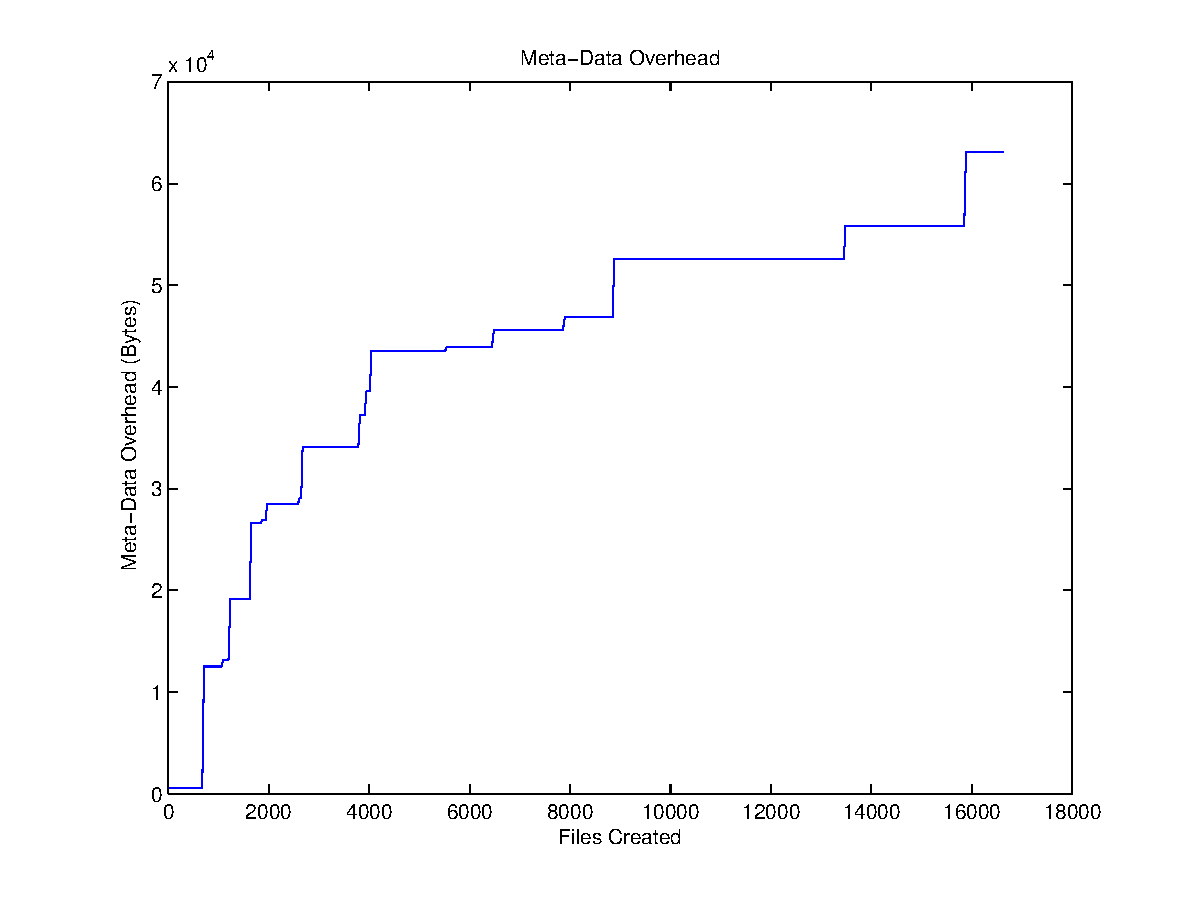
\includegraphics[width=4.5in]{metadata.eps}
\caption{{\bf MetaData OVerhead}.  This figure shows the size of TnT's metadata as the number of files created in the distributed system is increased.  The curve is sub-linear because metadata is proportional to the number of files in the system and not the number of files created.  When files are deleted, they are removed from the metadata.}
\label{fig:metadata}
\end{figure}

\end{itemize}
